\chapter{Mengenal Kecerdasan Buatan dan
Scikit-Learn}
\section{Teori}
\subsection{ Definisi, Sejarah dan perkembangan Kecerdasan Buatan}
\paragraph{Definisi}: Kecerdasan buatan adalah bagaimana sistem untuk bisa cepat dan tepat, mencari dengan waktu yang sangat singkat untuk mendapatkan hasil dari sebuah keputusan, pencarian, dan pengelompokan.
\paragraph{Sejarah}:
\begin{itemize}
    \item Era komputer elektronik (1941) \\
    Ditemukannya pertama kali alat penyimpanan dan pemrosesan informasi yang yaitu komputer elektronik. Penemuan ini menjadi dasar pengembangan program yang mengarah ke kecerdasan buatan.
    
    \item Masa persiapan AI (1943-1956) \\
    Pada 1943, Warren McCulloch dan Walter Pitts berhasil membuat suatu model saraf tiruan di mana setiap neuron digambarkan sebagai ‘on’ dan ‘off’. Mereka menunjukkan bahwa setiap fungsi dapat dihitung dengan suatu jaringan sel saraf dan bahwa semua hubungan logis dapat diimplementasikan dengan struktur jaringan yang simple.
    Pada tahun 1950, Norbert Wiener melakukan penelitian mengenai prinsip-prinsip teori feedback. Contoh terkenal adalah thermostat.
    
    \item Awal perkembangan (1952-1969) \\
    Pada tahun 1958, McCarthy di MIT AI Lab mendefinisikan bahasa pemrograman tingkat tinggi yaitu LISP.
    Pada tahun 1959, Program komputer General Problem Solver berhasil dibuat oleh Herbert A. Simon, J.C. Shaw, dan Allen Newell. Program ini dirancang untuk memulai penyelesaian masalah secara manusiawi.
    Pada tahun 1963, program yang dibuat James Slagle mampu menyelesaikan masalah integral tertutup untuk mata kuliah Kalkulus.
    Pada tahun 1968, program analogi buatan Tom Evan menyelesaikan masalah analogi geometri yang ada pada tes IQ.
    
    \item Perkembangan AI melambat (1966-1974) \\
    Perkembangan AI melambat disebabkan adanya beberapa kesulitan yang di hadapi seperti  Program-program AI yang bermunculan hanya mengandung sedikit atau bahkan tidak mengandung sama sekali pengetahuan pada subjeknya
    
    \item Sistem berbasis pengetahuan (1969-1979) \\
    Pada tahun 1960an, Ed Feigenbaum, Bruce Buchanan, dan Joshua Lederberg merintis proyek DENDRAL yaitu program untuk memecahkan masalah struktur molekul dari informasi yang didapatkan dari spectometer massa.
    
    \item AI menjadi sebuah industry (1980-1988) \\
    Industralisasi AI diawali dengan ditemukannya sistem pakar yang dinamakan R1 yang mampu mengkonfigurasi sistem-sistem komputer baru. Program tersebut mulai dioperasikan di Digital Equipment Corporation (DEC), McDermott, pada tahun 1982.
    
    \item Kembalinya jaringan saraf tiruan (1986 – sekarang) \\
    Ahli fisika seperti Hopfield (1982) menggunakan teknik-teknik mekanika statistika untuk menganalisa sifat-sifat penyimpanan dan optimasi pada jaringan saraf. Para ahli psikolog, David Rumhelhart dan Geoff Hinton melanjutkan penelitian mengenai model jaringan saraf pada memori. Pada tahun 1985-an sedikitnya empat kelompok riset menemukan algoritma Back-Propagation. Algoritma ini berhasil diimplementasikan ke dalam ilmu bidang komputer dan psikologi.
\end{itemize}

 \paragraph{Perkembangan AI}Contoh tren Artificial Intelligence yang diprediksi akan mendongkrak perkembangan bisnis adalah sebagai berikut :
 \begin{itemize}
     \item Rekomendasi Cerdas, Melalui rekomendasi cerdas, Anda akan mendapatkan rekomendasi produk dan layanan yang cocok dengan kebutuhan pribadi Anda. Rekomendasi cerdas ini diperoleh berdasarkan analisa data dan pengalaman belanja pelanggan yang dimiliki oleh pebisnis online.
     
     \item Asisten Fiktif/ Virtual, Jadi, asisten virtual ini dirancang untuk menjawab pertanyaan dari pelanggan, melakukan percakapan layaknya manusia dan melaksanakan perintah yang diajukan oleh pelanggan.
     
     \item Speech Recognition, Tujuan perusahaan yang menerapkan speech recognition tersebut adalah untuk membantu pelanggan untuk bisa mendapatkan informasi, layanan dan juga produk yang diinginkan.
     
     \item Keamanan Digital, Dengan ditambahkannya AI pada sistem keamanan digital nantinya diharapkan akan mampu mendeteksi  aktivitas-aktivitas yang menyimpang pada sistem perusahaan.
 \end{itemize}
 
 \subsection{Resume mengenai definisi supervised learning, klasifikasi, regresi dan unsupervised learning. Data set, training set dan testing set.}
 \begin{enumerate}
     \item SUPERVISED LEARNING \\
      Supervised learning merupakan sebuah pembelajaran yang terawasi dimana jika output yang diharapkan telah diketahui sebelumnya. Biasanya pembelajaran ini dilakukan dengan menggunakan data yang telah ada. Pada metode ini, setiap pola yang diberikan kedalam jaringan saraf tiruan telah diketahui outputnya.
      
      \item Klasisfikasi \\
      klasifikasi adalah proses untuk menemukan model atau fungsi yang menjelaskan atau membedakan konsep atau kelas data, dengan tujuan untuk dapat memperkirakan kelas dari suatu objek yang labelnya tidak diketahui.
      
      \item Regresi \\
      Regresi adalah fungsi pembelajaran yang memetakan sebuah unsur data ke sebuah tabel prediksi bernilai nyata.
      
      \item Unsupervised learning \\
      merupakan pembelajan yang tidak terawasi dimana tidak memerlukan target output. 
      
      \item Training set \\
      adalah bagian dataset yang kita latih untuk membuat prediksi atau menjalankan fungsi dari sebuah algoritma ML. Kita memberikan petunjuk melalui algoritma agar mesin yang kita latih bisa mencari korelasinya sendiri atau belajar pola dari data yang diberikan.
      
      \item Testing set \\
      dalah bagian dataset yang kita tes untuk melihat keakuratannya, atau dengan kata lain melihat performanya.
      Sekarang kita akan belajar cara membagi dataset menjadi training dan test set dengan bahasa python dan R.
 \end{enumerate}
 \section{Instalasi}
\begin{enumerate}
    \item Instalasi library scikit dari anaconda, mencoba kompilasi dan uji coba ambil contoh kode dan lihat variabel explorer! \\
    
    \begin{figure}[!htbp]
        \centering
        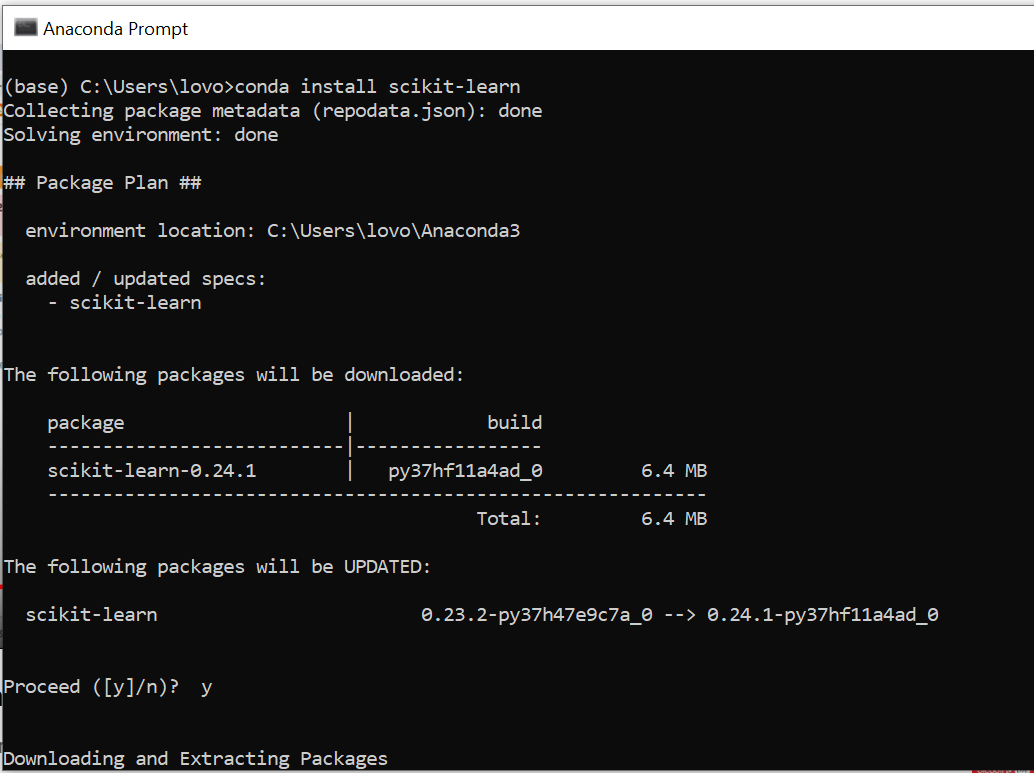
\includegraphics [width=8cm]{figures/instal_scikit.PNG}
        \caption{Instalasi Scikit-learn}
        \label{fig:my_label}
        \end{figure}
    
    \item Mencoba Loading an example dataset, menjelaskan maksud dari tulisan tersebut dan mengartikan per baris !
    
     \begin{figure}[!htbp]
        \centering
        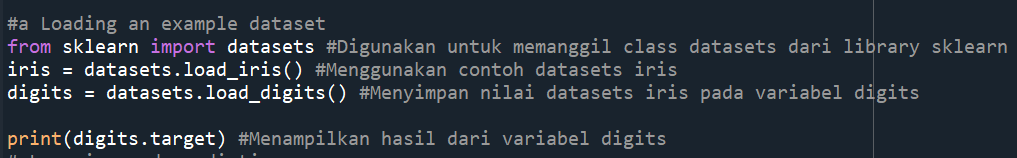
\includegraphics [width=8cm]{figures/Loadingdataset.PNG}
        \caption{Loading an example dataset}
        \label{fig:my_label}
        \end{figure}
        
    \item Mencoba Learning and predicting, menjelaskan maksud dari tulisan tersebut dan mengartikan per baris !
    
     \begin{figure}[!htbp]
        \centering
        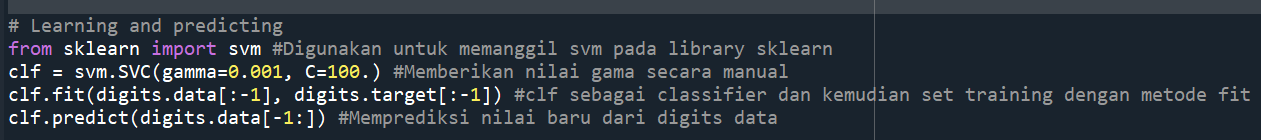
\includegraphics [width=8cm]{figures/Learningandpredicting.PNG}
        \caption{Learning and predicting}
        \label{fig:my_label}
        \end{figure}
        
    \item Mencoba Model persistence, menjelaskan maksud dari tulisan tersebut dan mengartikan per baris ! \\
    
     \begin{figure}[!htbp]
        \centering
        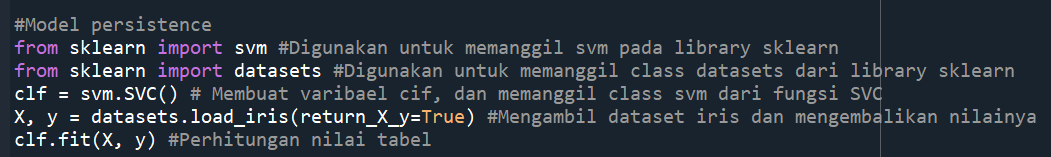
\includegraphics [width=8cm]{figures/Modelpresistence.PNG}
        \caption{Model presistence}
        \label{fig:my_label}
        \end{figure}
        
    \item Mencoba Conventions, menjelaskan maksud dari tulisan tersebut dan mengartikan per baris !
    
      \begin{figure}[!htbp]
        \centering
        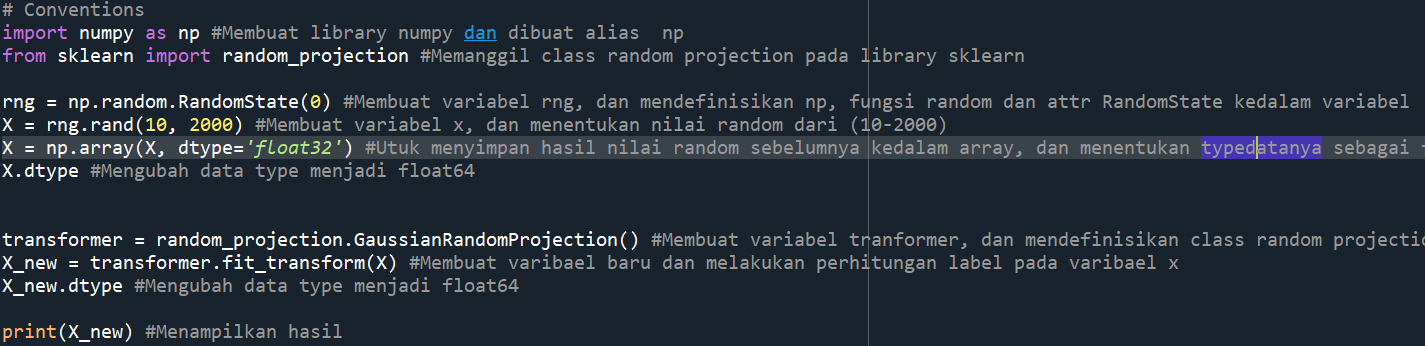
\includegraphics [width=8cm]{figures/Conventions.PNG}
        \caption{Conventions}
        \label{fig:my_label}
        \end{figure}
    
\end{enumerate}